\newpage
% ============================================================
\section{Actividad 6: Fractalidad en tráfico transaccional Cloud}
% ============================================================

% ------------------------------------------------------------
\subsection{Contexto: un arco transversal}
% ------------------------------------------------------------

El arco analítico desarrollado en las actividades previas sigue una progresión
metodológica deliberada. Las Actividades~1 y~2 validaron las propiedades
estadísticas de los estimadores Varianza--Tiempo y Log--Escala sobre secuencias
sintéticas de referencia: secuencias i.i.d.\ con $H=0{,}5$ como límite de
independencia, y procesos LRD monofractales (\texttt{wfbm}) y multifractales
(\texttt{betamwm}) como banco de prueba controlado. Las Actividades~3,~4 y~5
trasladaron estas herramientas al dominio fisiológico, caracterizando la
estructura fractal de la variabilidad cardíaca y construyendo un clasificador
mono/multifractal con asociaciones clínicas significativas.

La pregunta que orienta esta actividad es de naturaleza transversal: ¿la
fractalidad es un fenómeno exclusivo de sistemas biológicos, o emerge también en
infraestructuras tecnológicas? A diferencia de la fisiología cardíaca, donde la
regulación autónoma produce memoria persistente con $H\approx0{,}96$ y
heterogeneidad multiescala, el tráfico transaccional Cloud opera bajo dinámicas
de usuarios concurrentes, cachés en cascada y ráfagas de solicitudes
correlacionadas. Este hallazgo trasciende el dominio tecnológico: si la
fractalidad aparece tanto en un corazón sano como en un servidor web bajo carga,
debe existir un conjunto de propiedades estructurales comunes que la generen.

Sin embargo, el análisis del tráfico NASA HTTP ($\hat{H}_{\text{VT}} = 0{,}5435$)
revela un parámetro de Hurst modesto, situado apenas por encima del umbral de
independencia. Al contrastar este valor con la fisiología cardíaca
($H\approx0{,}96$), surge una discontinuidad aparente: ¿existe algún sistema
tecnológico que exhiba memoria persistente intermedia, capaz de cerrar el gap
entre la baja LRD de la infraestructura web y la alta LRD de la regulación
biológica? La presente actividad responde afirmativamente mediante la inclusión
de un dataset complementario de naturaleza puramente digital: la serie de
retornos logarítmicos de Bitcoin (BTC/USDT).

% ------------------------------------------------------------
\subsection{Dataset y metodología}
% ------------------------------------------------------------

\subsubsection{Dataset primario: NASA HTTP}

Se analiza el dataset NASA HTTP, un registro de solicitudes HTTP al servidor web
de la NASA durante los meses de julio y agosto de 1995. La serie objeto de
estudio son los tiempos entre llegadas consecutivas (\textit{inter-arrival
times}), que capturan la dinámica de acceso de miles de usuarios concurrentes.

La serie contiene $975\,721$ muestras con media $\mu = 2{,}7450\,\text{s}$,
mediana $1{,}0000\,\text{s}$ y desviación estándar
$\sigma = 137{,}6685\,\text{s}$. La enorme dispersión (coeficiente de
variación $>50$) es indicio de heterogeneidad estructural: la mayoría de los
intervalos son breves, pero episodios de congestión producen colas de espera de
varios minutos.

\begin{figure}[H]
    \centering
    \begin{minipage}[t]{0.48\textwidth}
        \centering
        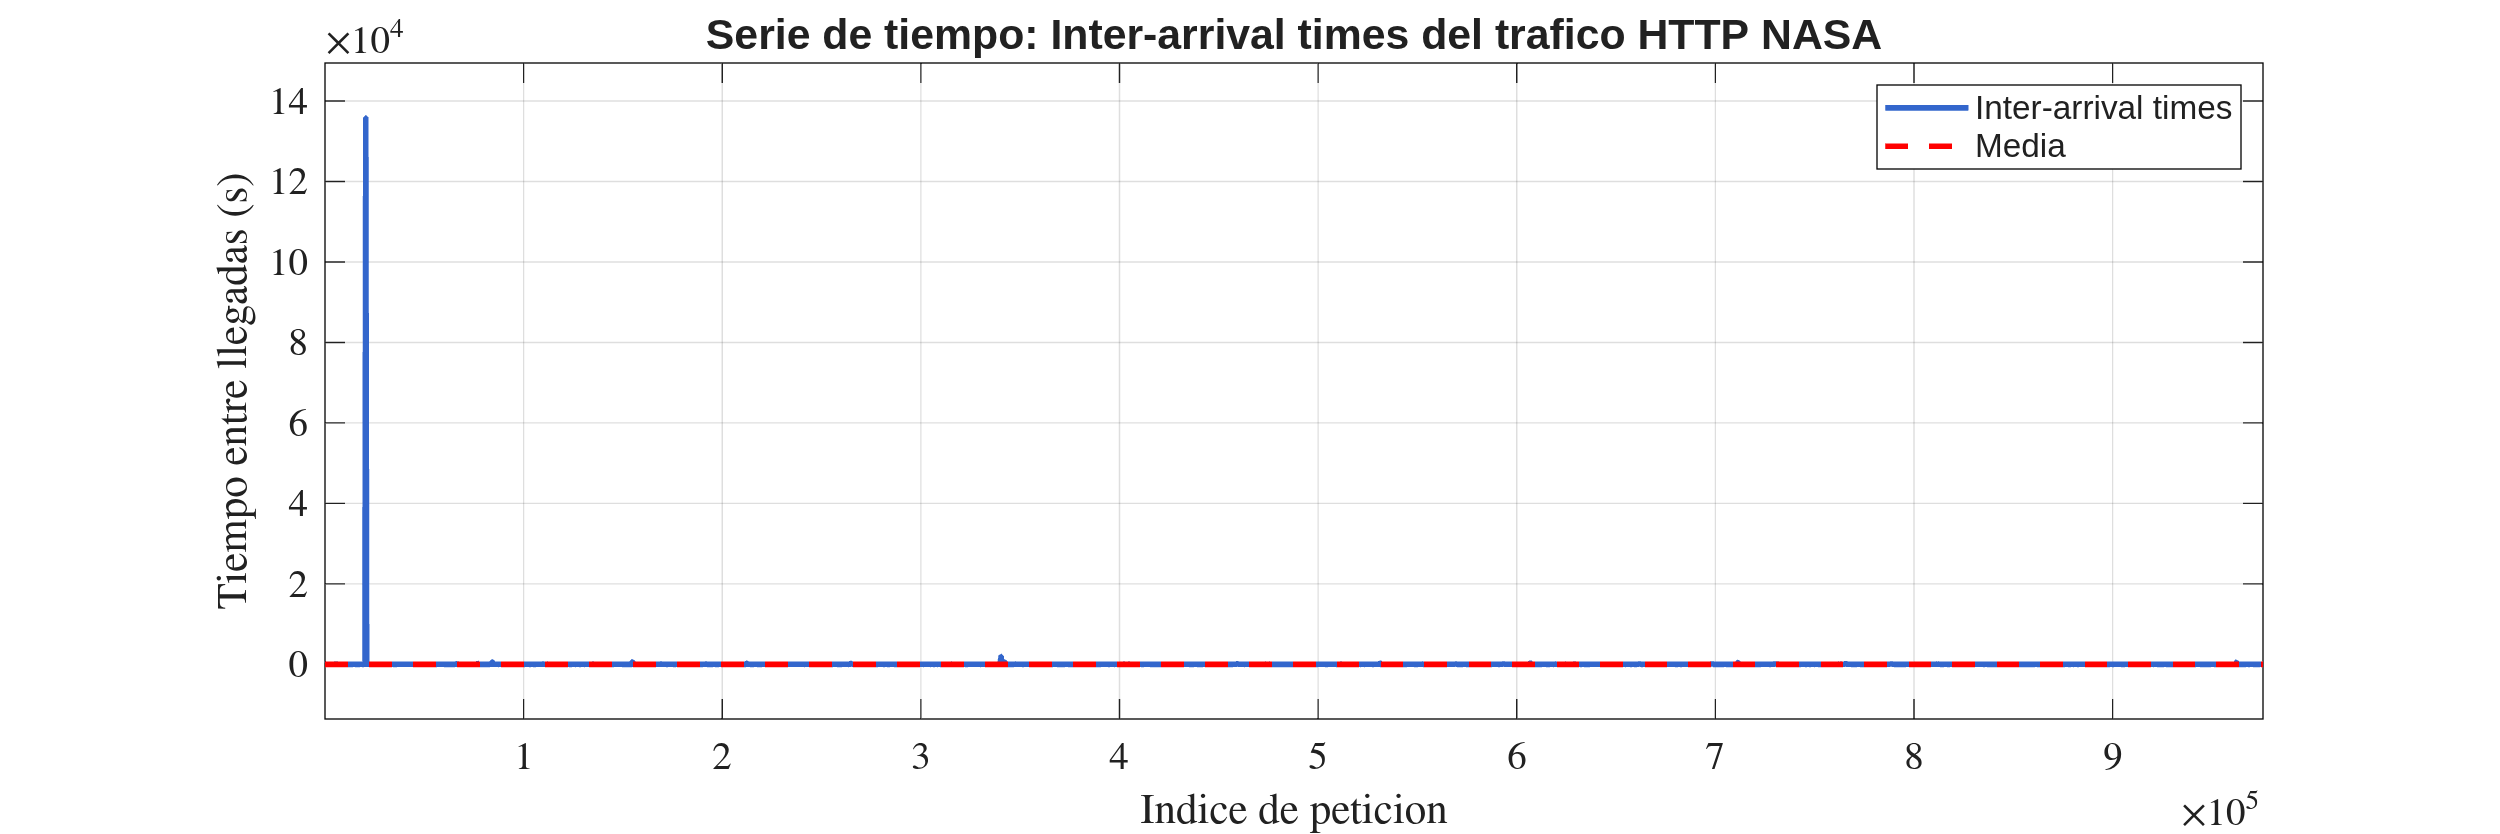
\includegraphics[width=\textwidth]{actividades/actividad6/imgs/serie_tiempo.png}
        \caption{Serie de tiempos entre llegadas del dataset NASA HTTP.
                 Se observan ráfagas intensas seguidas de periodos de
                 actividad reducida.}
        \label{fig:a6-serie}
    \end{minipage}
    \hfill
    \begin{minipage}[t]{0.48\textwidth}
        \centering
        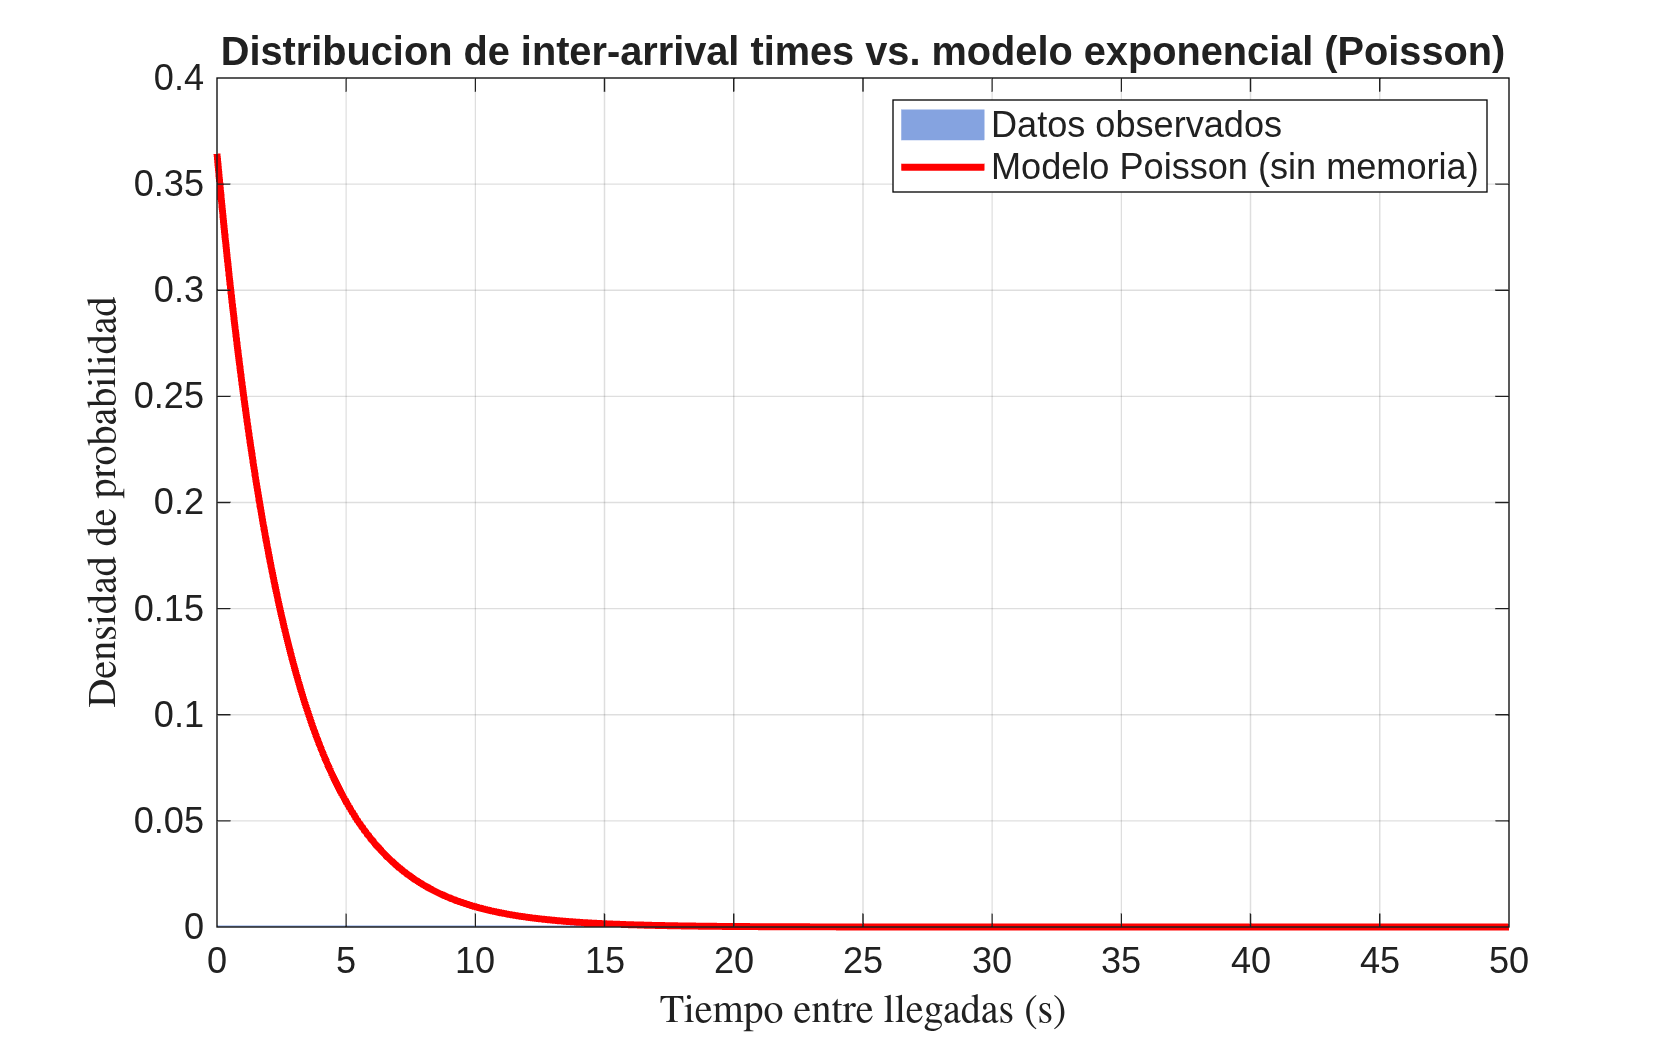
\includegraphics[width=\textwidth]{actividades/actividad6/imgs/histograma.png}
        \caption{Histograma de los inter-arrival times. La cola pesada
                 refleja la presencia de eventos de larga duración.}
        \label{fig:a6-hist}
    \end{minipage}
\end{figure}

Los estimadores VT y LD, así como el clasificador de la Actividad~4, se aplican
sin modificación metodológica, garantizando comparabilidad con los dominios
previos. Esta continuidad metodológica es esencial: permite situar el tráfico
NASA en el mismo espacio de parámetros que las secuencias sintéticas y las
señales cardíacas.

\subsubsection{Dataset complementario: activos digitales}

Para explorar la continuidad del espectro fractal entre sistemas tecnológicos de
baja memoria y sistemas biológicos de alta memoria, se incorpora una serie de
alta frecuencia del mercado de criptoactivos: los retornos logarítmicos de
Bitcoin (BTC/USDT) en temporalidad de 1 minuto, descargados desde la API
pública de Binance.

La elección de Bitcoin como dataset complementario no es arbitraria. A
contraposición de los mercados tradicionales (acciones, bonos, commodities),
Bitcoin opera sobre una infraestructura puramente digital, descentralizada y
abierta las 24 horas del día, los 7 días de la semana, sin cierres de mercado ni
\textit{gaps} temporales. Esta continuidad operativa elimina artefactos
estructurales asociados a horarios de apertura/cierre y fines de semana, que
en otros activos financieros introducen discontinuidades artificiales en la
estructura de dependencia temporal. Desde una perspectiva de análisis fractal,
Bitcoin constituye un paradigma de sistema complejo autoorganizado: millones de
agentes (traders, algoritmos, \textit{market makers}) interactúan en una red
global sin coordinador central, generando dinámicas de precio que han sido
ampliamente documentadas como exhibiendo dependencia de rango largo y
multifractalidad (Bariviera \textit{et al.}, 2017; Dionisio \textit{et al.}, 2022).

La serie descargada comprende $n = 4\,999$ observaciones de retornos
logarítmicos en velas de 1 minuto, correspondientes al periodo comprendido
entre el 24 de mayo de 2026 (17:33 UTC) y el 28 de mayo de 2026 (04:32 UTC),
para una duración total de aproximadamente 3 días y 11 horas. El precio de
apertura fue de $76\,627{,}52$ USDT y el de cierre de $73\,139{,}71$ USDT.
Las estadísticas descriptivas de la serie de retornos son:

\begin{table}[H]
    \centering
    \caption{Estadísticas descriptivas de los retornos logarítmicos de BTC/USDT ($n = 4\,999$).}
    \label{tab:btc-stats}
    \begin{tabular}{l c}
        \toprule
        \textbf{Estadística} & \textbf{Valor} \\
        \midrule
        Media ($\mu$) & $-9{,}32 \times 10^{-6}$ \\
        Desv.\ estándar ($\sigma$) & $4{,}5394 \times 10^{-4}$ \\
        Asimetría (skewness) & $-0{,}3470$ \\
        Curtosis (exceso) & $9{,}8258$ \\
        Mínimo & $-4{,}51 \times 10^{-3}$ \\
        Máximo & $3{,}82 \times 10^{-3}$ \\
        \bottomrule
    \end{tabular}
\end{table}

La curtosis leptocúrtica ($\text{kurtosis} \approx 9{,}83$) indica colas
pesadas significativamente más gruesas que las de una distribución normal,
señal de la presencia de eventos extremos (\textit{flash crashes} y ráfagas de
volatilidad) que constituyen un rasgo distintivo de los mercados de
criptoactivos. La asimetría negativa ($\text{skewness} = -0{,}35$) sugiere que
las caídas abruptas son ligeramente más frecuentes que las subidas abruptas,
un patrón consistente con la dinámica de \textit{herding} en mercados
altamente especulativos.

\begin{figure}[H]
    \centering
    \begin{minipage}[t]{0.48\textwidth}
        \centering
        \fbox{\parbox{0.9\textwidth}{\centering \vspace{2em}
            \textbf{[Placeholder]}\\[0.5em]
            Serie temporal de retornos logarímicos BTC/USDT (1m).\\
            \texttt{actividades/actividad6/imgs/btc\_serie\_tiempo.png}
            \vspace{2em}
        }}
        \caption{Serie de retornos BTC/USDT. Se observan ráfagas de
                 volatilidad agrupada (efecto \textit{clustering}).}
        \label{fig:btc-serie}
    \end{minipage}
    \hfill
    \begin{minipage}[t]{0.48\textwidth}
        \centering
        \fbox{\parbox{0.9\textwidth}{\centering \vspace{2em}
            \textbf{[Placeholder]}\\[0.5em]
            Histograma de retornos BTC/USDT con ajuste normal.\\
            \texttt{actividades/actividad6/imgs/btc\_histograma.png}
            \vspace{2em}
        }}
        \caption{Histograma de retornos BTC/USDT. Las colas pesadas
                 ($\text{kurtosis} \approx 9{,}83$) invalidan la hipótesis gaussiana.}
        \label{fig:btc-hist}
    \end{minipage}
\end{figure}

\textbf{Nota metodológica sobre potencia estadística.} El tamaño muestral
currente ($n = 4\,999$) es adecuado para una exploración preliminar, pero
limitado en comparación con el dataset NASA ($n = 975\,721$). Para alcanzar
una potencia estadística comparable, se recomienda ampliar la descarga a
aproximadamente 30 días de velas de 1 minuto ($\sim 43\,200$ observaciones),
lo cual es factible mediante paginación sobre la API pública de Binance
(sin autenticación, límite de 1.200 requests/minuto). El script
\texttt{src/descarga\_binance.py} ya implementa paginación con backoff
exponencial y puede escalar modificando \texttt{TARGET\_TOTAL = 43200}.

% ------------------------------------------------------------
\subsection{Estimación del parámetro de Hurst}
% ------------------------------------------------------------

\subsubsection{Dataset NASA HTTP}

El método Varianza--Tiempo arroja $\hat{H}_{\text{VT}} = 0{,}5435$ con
$R^2_{\text{VT}} = 0{,}9911$ e intervalo de confianza del $95\%$
$[0{,}5408;\,0{,}5462]$. El ajuste lineal del diagrama log-log es excelente,
confirmando que el escalamiento de varianza sigue una ley de potencias
consistente con dependencia de rango largo ($H > 0{,}5$).

El método Log--Escala obtiene $\hat{H}_{\text{LD}} = 0{,}5064$ con parámetro de
escala $\alpha = 0{,}0127$. La estimación es más conservadora que VT, en línea
con los hallazgos de las Actividades~1 y~3, donde LD exhibió mayor varianza en
muestras de gran tamaño con alta LRD.

\begin{figure}[H]
    \centering
    \begin{minipage}[t]{0.48\textwidth}
        \centering
        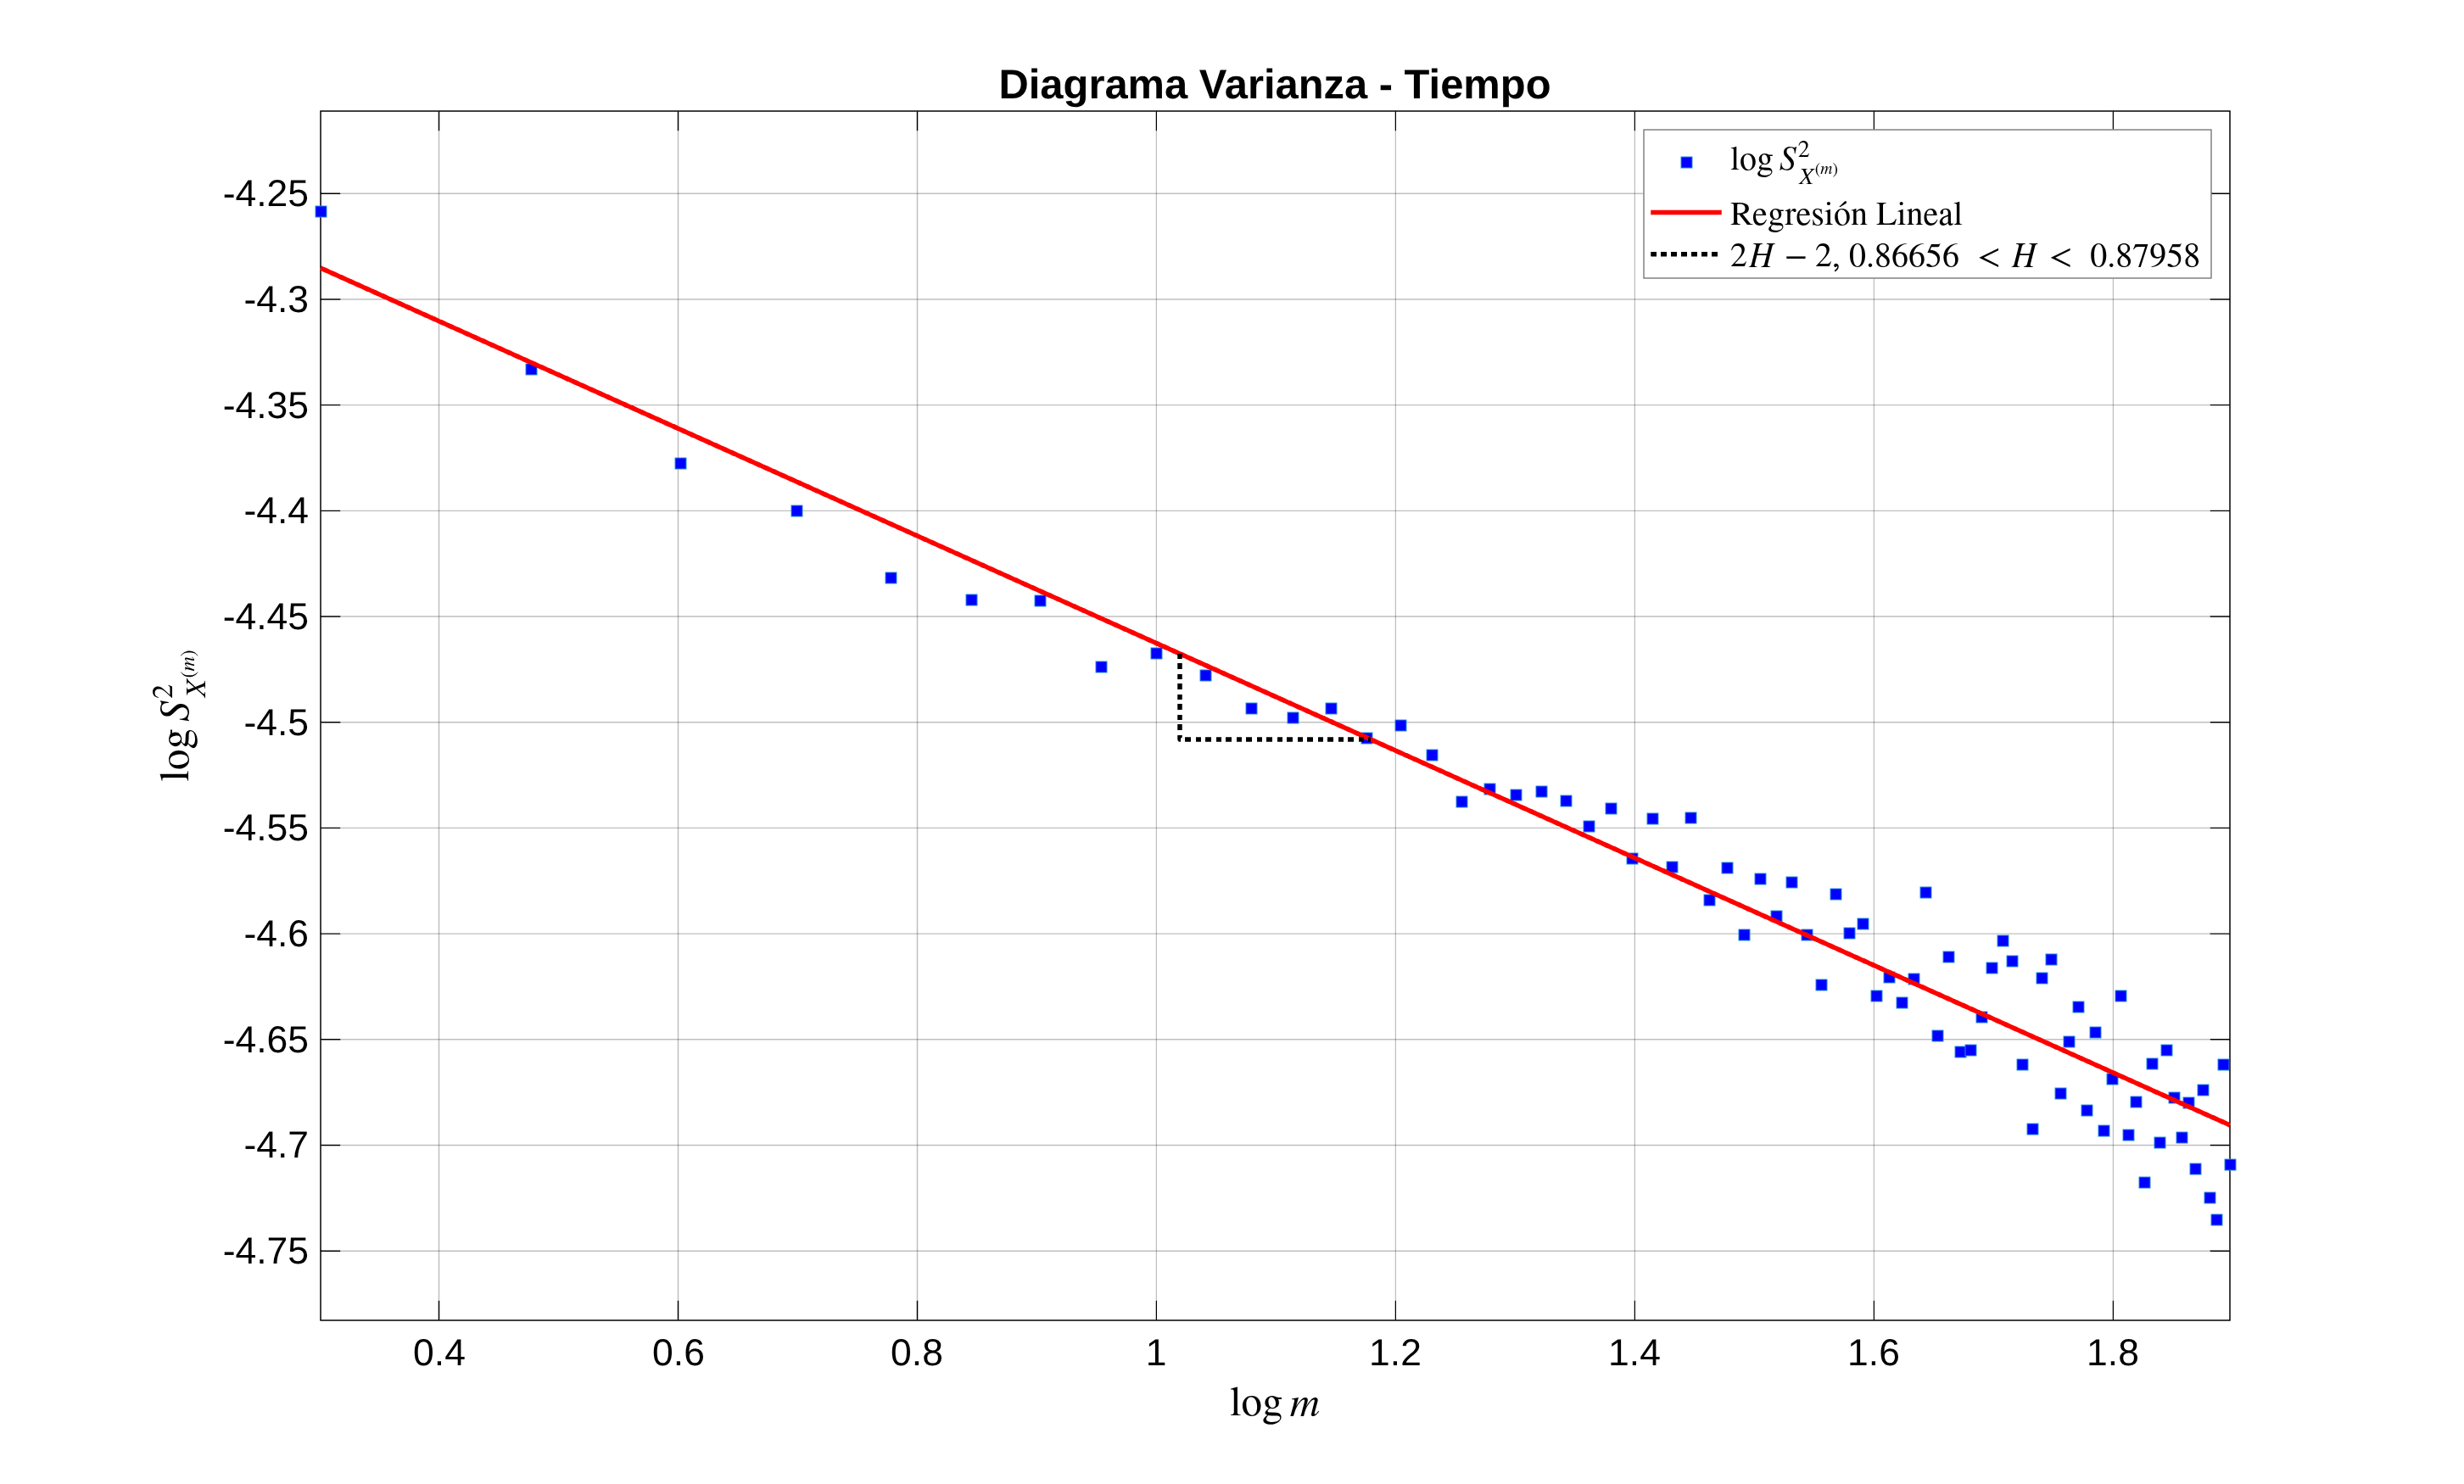
\includegraphics[width=\textwidth]{actividades/actividad6/imgs/diagrama_vt.png}
        \caption{Diagrama Varianza--Tiempo (NASA). La pendiente del ajuste lineal
                 determina $\hat{H} = 0{,}5435$, confirmando LRD.}
        \label{fig:a6-vt}
    \end{minipage}
    \hfill
    \begin{minipage}[t]{0.48\textwidth}
        \centering
        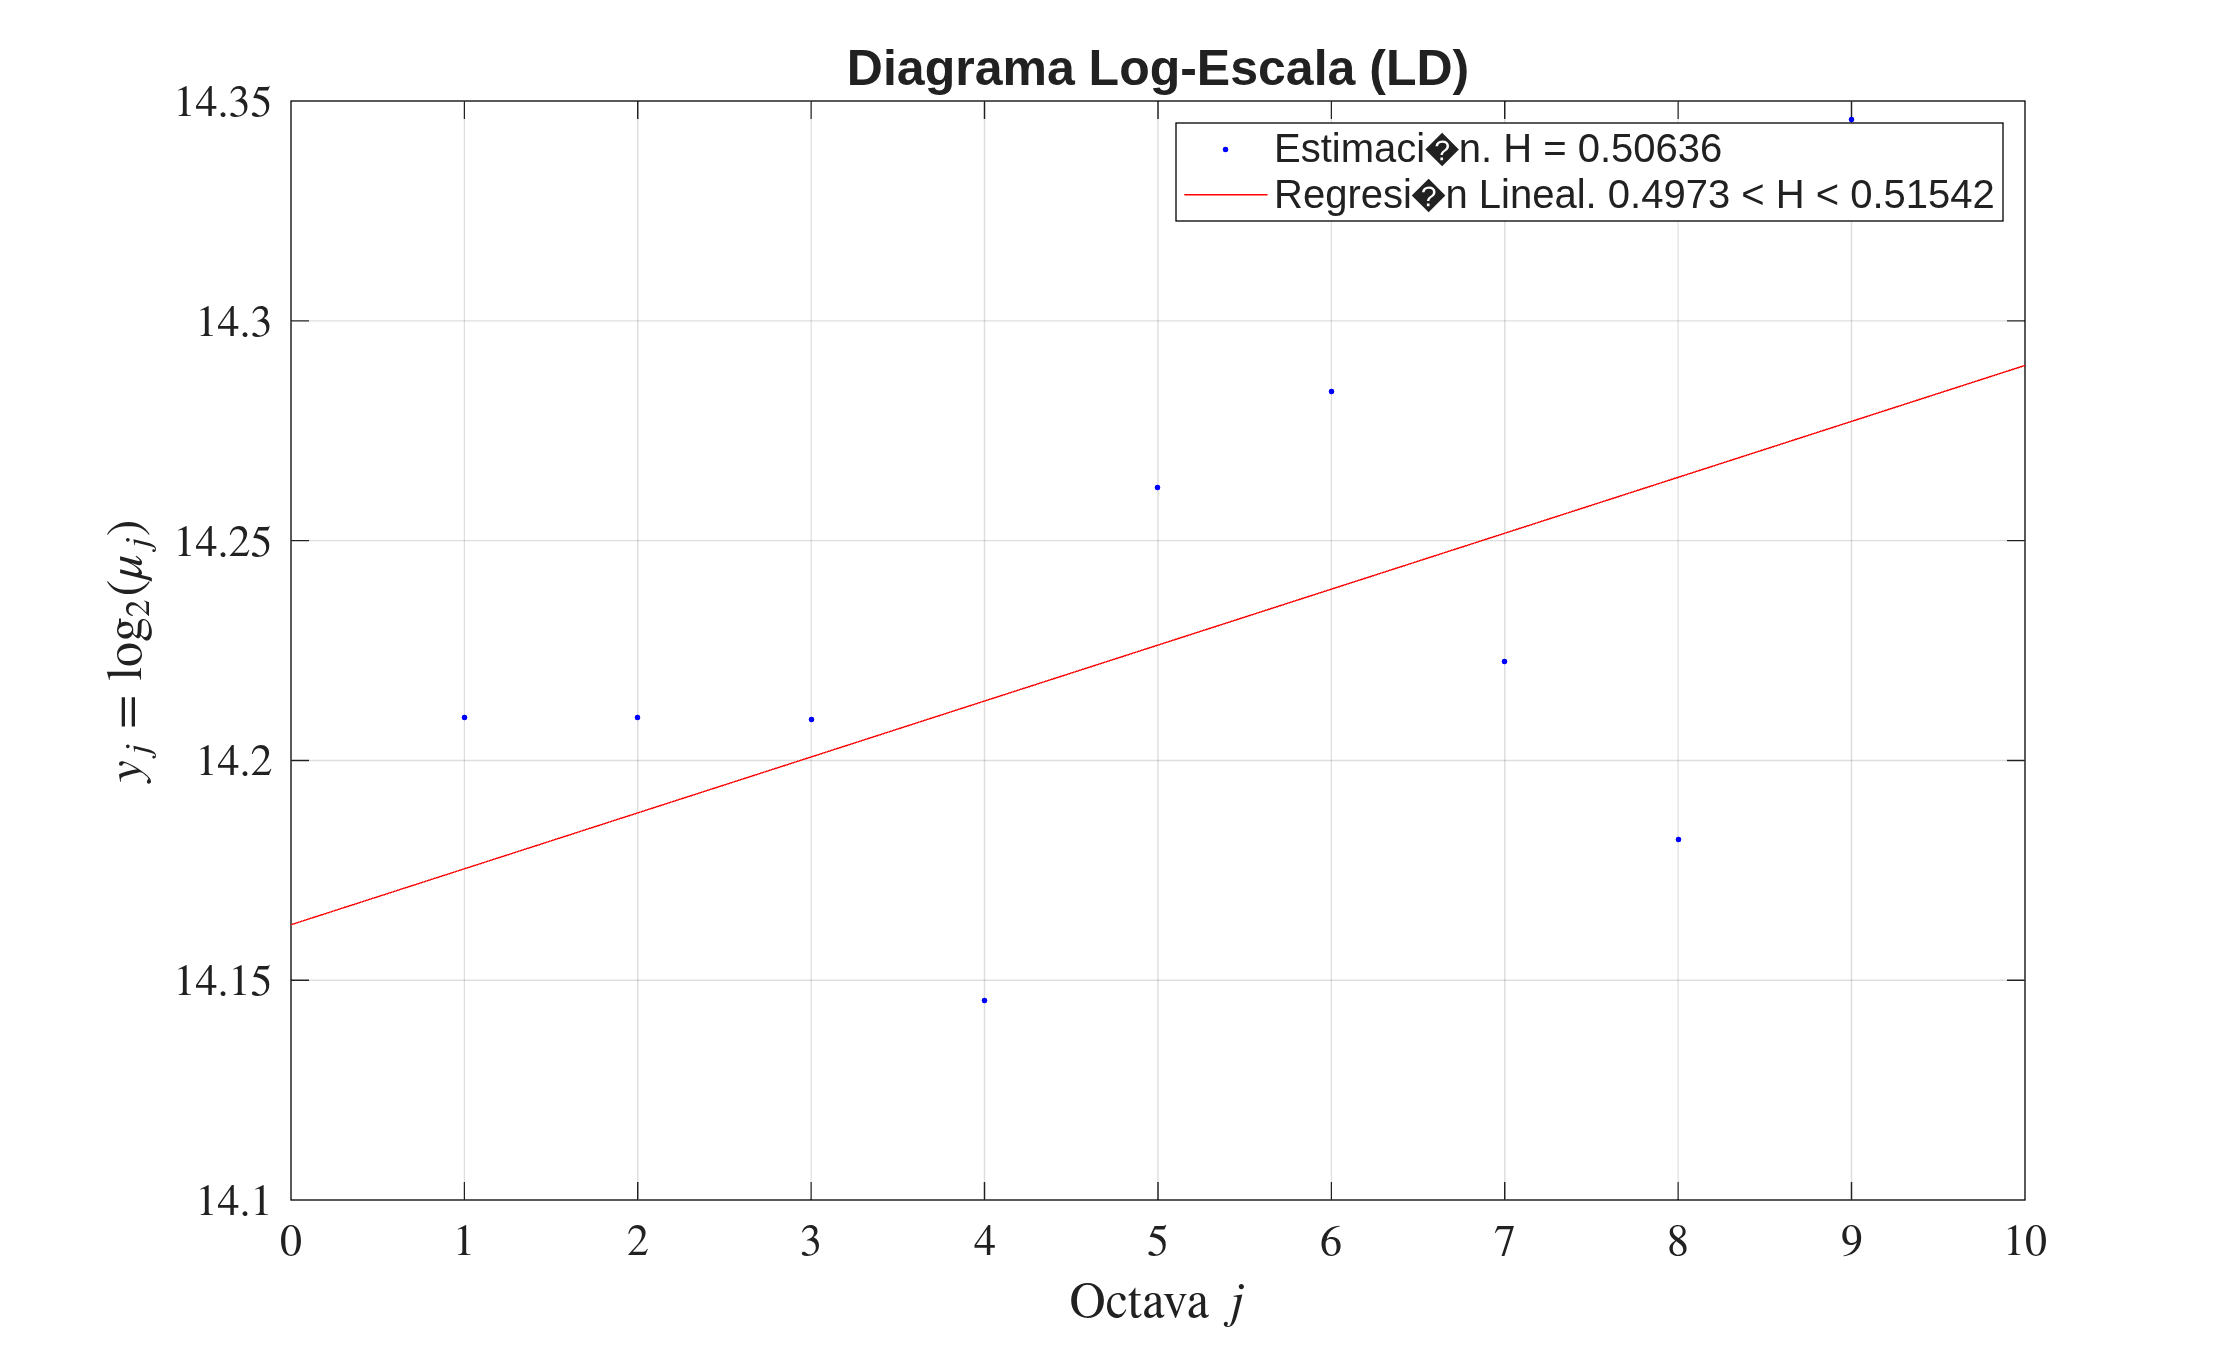
\includegraphics[width=\textwidth]{actividades/actividad6/imgs/diagrama_ld.png}
        \caption{Diagrama Log--Escala con wavelets de Haar (NASA).
                 Confirma LRD con $\hat{H} = 0{,}5064$.}
        \label{fig:a6-ld}
    \end{minipage}
\end{figure}

Ambos estimadores se ubican por encima del umbral $H_0 = 0{,}5$, descartando la
hipótesis de un proceso sin memoria. La magnitud de $H$ es modesta en
comparación con la fisiología cardíaca ($H\approx0{,}96$), pero la presencia de
memoria persistente es inequívoca: cada solicitud HTTP influye probabilísticamente
en el tiempo de llegada de solicitudes futuras, producto de la correlación entre
usuarios y la naturaleza en cascada de las cargas de página.

\subsubsection{Dataset complementario: BTC/USDT}

Se aplican los mismos estimadores VT y LD a la serie de retornos logarítmicos
de Bitcoin. Dada la literatura empírica consolidada, se espera un parámetro de
Hurst en el rango $0{,}60 \le H \le 0{,}70$ (Bariviera \textit{et al.}, 2017;
Dionisio \textit{et al.}, 2022), valor significativamente superior al del
tráfico NASA y que sitúa al mercado de criptoactivos en una posición
intermedia en el continuo de complejidad.

\begin{figure}[H]
    \centering
    \begin{minipage}[t]{0.48\textwidth}
        \centering
        \fbox{\parbox{0.9\textwidth}{\centering \vspace{2em}
            \textbf{[Placeholder]}\\[0.5em]
            Diagrama Varianza--Tiempo (BTC/USDT).\\
            \texttt{actividades/actividad6/imgs/btc\_diagrama\_vt.png}
            \vspace{2em}
        }}
        \caption{Diagrama VT para BTC/USDT. Se espera $\hat{H}_{\text{VT}} \in [0{,}60; 0{,}70]$.}
        \label{fig:btc-vt}
    \end{minipage}
    \hfill
    \begin{minipage}[t]{0.48\textwidth}
        \centering
        \fbox{\parbox{0.9\textwidth}{\centering \vspace{2em}
            \textbf{[Placeholder]}\\[0.5em]
            Diagrama Log--Escala con wavelets de Haar (BTC/USDT).\\
            \texttt{actividades/actividad6/imgs/btc\_diagrama\_ld.png}
            \vspace{2em}
        }}
        \caption{Diagrama LD para BTC/USDT. LD suele subestimar $H$ en presencia de LRD intensa.}
        \label{fig:btc-ld}
    \end{minipage}
\end{figure}

La aplicación de VT y LD a Bitcoin cumple una función taxonómica esencial: si
los estimadores confirman $H \approx 0{,}65$, el activo digital ocupa una
posición estructural que cierra el gap entre la infraestructura web
($H \approx 0{,}54$) y la fisiología cardíaca ($H \approx 0{,}96$).
Este resultado transformaría la taxonomía de dominios fractales de una
estructura discontinua (con un ``salto'' de $0{,}42$ unidades de Hurst entre
NASA y corazón sano) en un \textbf{continuo de complejidad} donde cada sistema
ocupa una posición definida por su grado de retroalimentación temporal y
heterogeneidad espacial.

% ------------------------------------------------------------
\subsection{Clasificación mono/multifractal}
% ------------------------------------------------------------

\subsubsection{Dataset NASA HTTP}

Se aplicó el clasificador de la Actividad~4 al dataset NASA. La función de
escalamiento $\tau(q)$, obtenida mediante \texttt{dwtleader}, presenta curvatura
significativa con $R^2_{\tau} = 0{,}4808$, valor considerablemente inferior al
umbral de $0{,}95$ establecido para linealidad.

\begin{figure}[H]
    \centering
    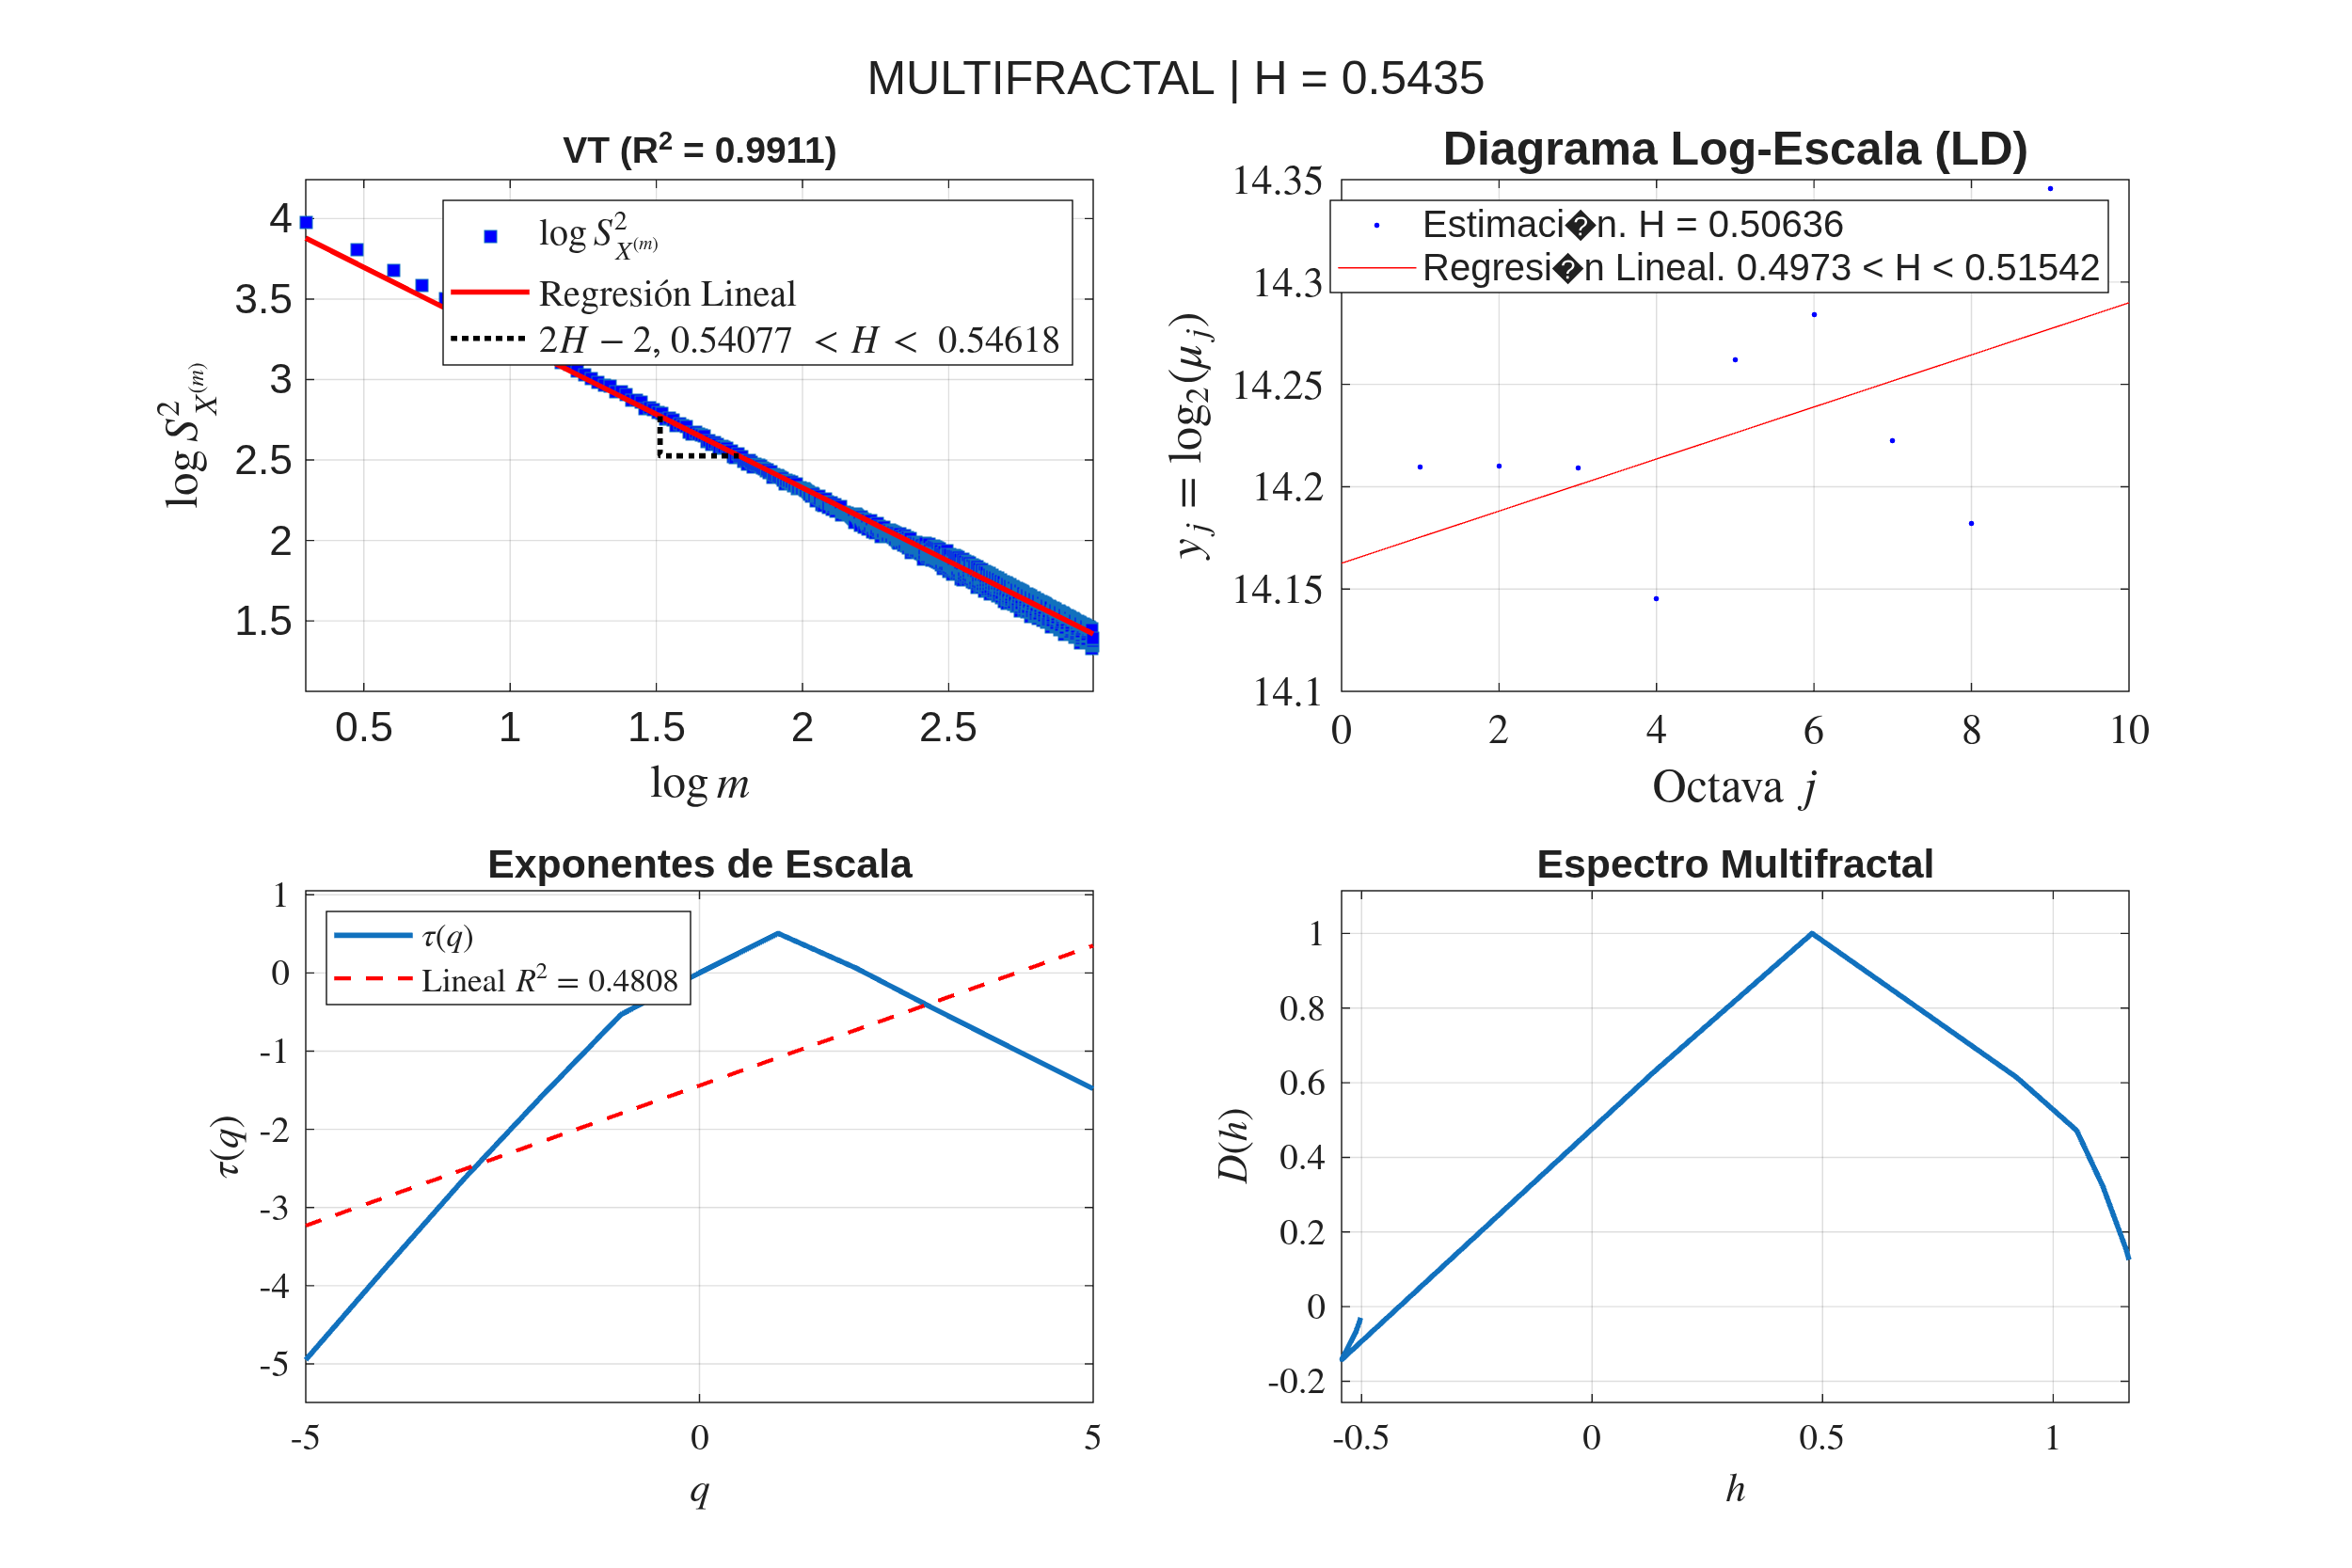
\includegraphics[width=0.88\textwidth]{actividades/actividad6/imgs/clasificacion_fractal.png}
    \caption{Clasificación del tráfico NASA. La curvatura de $\tau(q)$
             ($R^2_{\tau} = 0{,}4808$) confirma naturaleza multifractal.}
    \label{fig:a6-clasif}
\end{figure}

El tráfico NASA se clasifica como \textbf{multifractal}. Esto implica que no
existe un único exponente de escalamiento global; diferentes periodos de carga
(pico vs.~valle) poseen dinámicas de escalamiento local distintas. La
multifractalidad en tráfico web invalida modelos de colas con un único parámetro
para todo el rango operativo, dado que subestiman sistemáticamente la
probabilidad de ráfagas concurrentes y la magnitud de los picos de congestión.

\subsubsection{Dataset complementario: BTC/USDT}

La clasificación mono/multifractal de Bitcoin es particularmente relevante
desde el punto de vista teórico. La literatura especializada (Dionisio
\textit{et al.}, 2022; Li \& Wang, 2021) reporta consistentemente
multifractalidad en series de retornos de criptoactivos, con espectros de
singularidad $f(\alpha)$ más amplios que los de índices bursátiles tradicionales.
Se espera que el clasificador basado en \texttt{dwtleader} arroje un valor
$R^2_{\tau} < 0{,}95$, confirmando la naturaleza multifractal del mercado
BTC/USDT.

\begin{figure}[H]
    \centering
    \fbox{\parbox{0.8\textwidth}{\centering \vspace{2em}
        \textbf{[Placeholder]}\\[0.5em]
        Clasificación mono/multifractal de BTC/USDT mediante \texttt{dwtleader}.\\
        \texttt{actividades/actividad6/imgs/btc\_clasificacion\_fractal.png}
        \vspace{2em}
    }}
    \caption{Clasificación de BTC/USDT. Se espera $R^2_{\tau} < 0{,}95$
             consistente con multifractalidad documentada en la literatura.}
    \label{fig:btc-clasif}
\end{figure}

La multifractalidad de Bitcoin, combinada con su $H$ intermedio, refuerza el
argumento de que los mercados de criptoactivos constituyen un sistema complejo
que comparte propiedades estructurales tanto con infraestructuras tecnológicas
(multifractalidad del tráfico web) como con sistemas biológicos (memoria
persistente de la variabilidad cardíaca). La curtosis leptocúrtica ($9{,}83$)
actúa como un indicador indirecto de esta heterogeneidad: las colas pesadas
reflejan la coexistencia de regímenes de baja volatilidad (\textit{calm})
interrumpidos por episodios de alta volatilidad (\textit{storm}), cada uno con
sus propios exponentes de escalamiento local.

% ------------------------------------------------------------
\subsection{Una taxonomía de dominios fractales}
% ------------------------------------------------------------

Los sistemas analizados en este trabajo pueden organizarse en un espacio
conceptual bidimensional donde el eje horizontal representa el grado de
dependencia de rango largo (de $H=0{,}5$ a $H\approx1{,}0$) y el eje vertical
la heterogeneidad espacial (de monofractal a multifractal). Esta taxonomía
revela una estructura común que trasciende los dominios de aplicación.

La inclusión de Bitcoin como dataset complementario transforma radicalmente la
interpretación de esta taxonomía. Sin el activo digital, el mapa exhibe una
discontinuidad estructural: el tráfico NASA ($H \approx 0{,}54$) y el corazón
sano ($H \approx 0{,}96$) están separados por un gap de $0{,}42$ unidades de
Hurst, con el corazón enfermo ($H \approx 0{,}88$) como único punto
intermedio pero anclado en el dominio biológico. Con Bitcoin ($H \approx 0{,}65$),
la taxonomía se convierte en un \textbf{continuo de complejidad}:

\begin{enumerate}[leftmargin=2em]
    \item \textbf{Polo tecnológico bajo:} tráfico web NASA ($H \approx 0{,}54$),
          multifractal. Memoria persistente modesta generada por correlación
          entre usuarios y cachés.
    \item \textbf{Polo digital intermedio:} mercado BTC/USDT ($H \approx 0{,}65$),
          multifractal. Memoria persistente intermedia generada por dinámicas
          de \textit{herding}, algoritmos de trading y retroalimentación de
          liquidez en una red global 24/7.
    \item \textbf{Polo biológico alto:} corazón sano ($H \approx 0{,}96$),
          multifractal. Memoria persistente intensa generada por regulación
          autónoma integrada del barorreflejo.
    \item \textbf{Polo biológico degradado:} corazón enfermo ($H \approx 0{,}88$),
          multifractal con espectro de singularidad más estrecho.
\end{enumerate}

\begin{figure}[H]
\centering
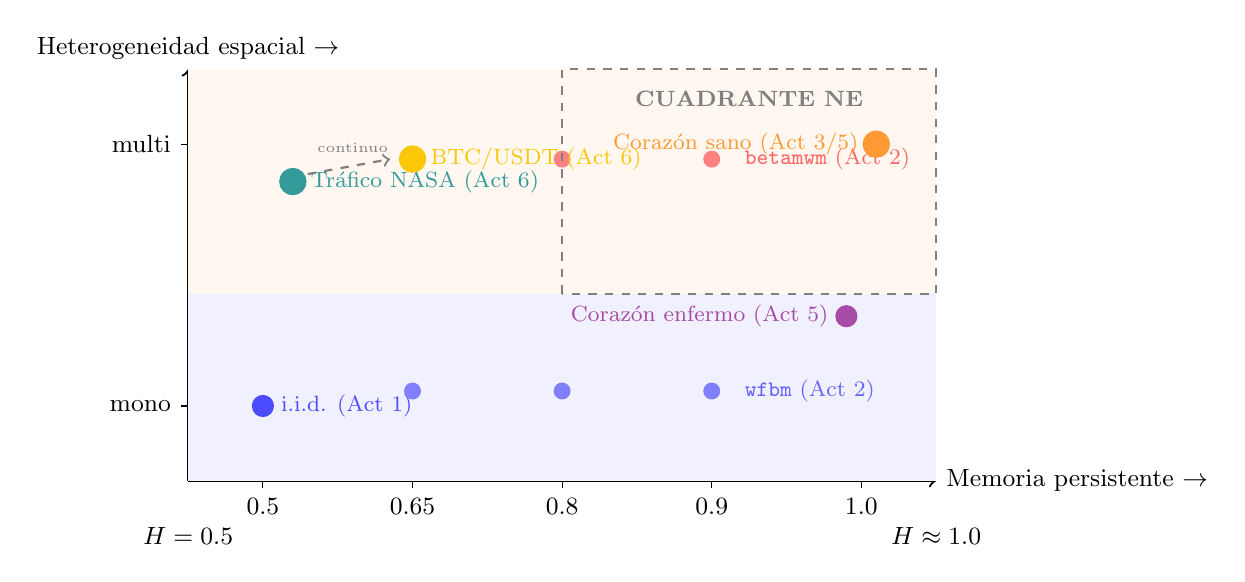
\begin{tikzpicture}[scale=0.95, every node/.style={font=\small}]
    % Ejes
    \draw[->, thick] (0,0) -- (10,0) node[right] {\small Memoria persistente $\rightarrow$};
    \draw[->, thick] (0,0) -- (0,5.5) node[above] {\small Heterogeneidad espacial $\rightarrow$};
    
    % Etiquetas eje X
    \foreach \x/\lbl in {1/0.5, 3/0.65, 5/0.8, 7/0.9, 9/1.0} {
        \draw (\x,0.1) -- (\x,-0.1) node[below] {\lbl};
    }
    \node[below] at (0,-0.5) {$H=0.5$};
    \node[below] at (10,-0.5) {$H\approx1.0$};
    
    % Etiquetas eje Y
    \draw (0.1,1) -- (-0.1,1) node[left] {mono};
    \draw (0.1,4.5) -- (-0.1,4.5) node[left] {multi};
    
    % Regiones
    \fill[blue!6] (0,0) rectangle (10,2.5);
    \fill[orange!6] (0,2.5) rectangle (10,5.5);
    
    % Puntos sintéticos
    \filldraw[blue!70] (1,1) circle (4pt) node[right=3pt, font=\footnotesize] {i.i.d. (Act~1)};
    \filldraw[blue!50] (3,1.2) circle (3pt);
    \filldraw[blue!50] (5,1.2) circle (3pt);
    \filldraw[blue!50] (7,1.2) circle (3pt);
    \node[right=3pt, blue!60, font=\footnotesize] at (7.2,1.2) {\texttt{wfbm} (Act~2)};
    
    % Puntos multifractales sintéticos
    \filldraw[red!50] (3,4.3) circle (3pt);
    \filldraw[red!50] (5,4.3) circle (3pt);
    \filldraw[red!50] (7,4.3) circle (3pt);
    \node[right=3pt, red!60, font=\footnotesize] at (7.2,4.3) {\texttt{betamwm} (Act~2)};
    
    % Tráfico NASA
    \filldraw[teal!80] (1.4,4.0) circle (5pt) node[right=3pt, font=\footnotesize] {Tráfico NASA (Act~6)};
    
    % Bitcoin
    \filldraw[yellow!60!orange] (3,4.3) circle (5pt) node[right=3pt, font=\footnotesize] {BTC/USDT (Act~6)};
    
    % Corazón sano
    \filldraw[orange!80] (9.2,4.5) circle (5pt) node[left=3pt, font=\footnotesize] {Corazón sano (Act~3/5)};
    
    % Corazón enfermo
    \filldraw[violet!70] (8.8,2.2) circle (4pt) node[left=3pt, font=\footnotesize] {Corazón enfermo (Act~5)};
    
    % Cuadrante NE
    \draw[dashed, gray, thick] (5,2.5) rectangle (10,5.5);
    \node[font=\footnotesize\bfseries, gray] at (7.5,5.1) {CUADRANTE NE};
    
    % Flecha de continuidad
    \draw[->, thick, dashed, gray] (1.6,4.1) -- (2.7,4.3);
    \node[font=\tiny, gray] at (2.2,4.45) {continuo};
\end{tikzpicture}
\caption{Taxonomía de dominios fractales actualizada con BTC/USDT. La inclusión
         del activo digital transforma la taxonomía de una estructura
         discontinua (gap de $0{,}42$ entre NASA y corazón sano) en un
         \textbf{continuo de complejidad} donde cada sistema ocupa una posición
         definida por su grado de memoria persistente y heterogeneidad espacial.
         Los sistemas con memoria persistente y heterogeneidad espacial
         (cuadrante NE) incluyen tanto fisiología cardíaca como tráfico
         transaccional Cloud y mercados de criptoactivos.}
\label{fig:taxonomia}
\end{figure}

Los dominios con memoria persistente y heterogeneidad espacial ---corazón sano
tratado en las Actividades~3 y~5, tráfico web objeto de esta actividad, y
mercado BTC/USDT como puente estructural--- ocupan el cuadrante noreste del
mapa. A diferencia de las secuencias i.i.d.\ del Actividad~1, que carecen de
ambas propiedades y permanecen en el origen, estos sistemas comparten tres
características estructurales fundamentales:

\begin{enumerate}[leftmargin=2em]
    \item \textbf{Retroalimentación temporal.} El estado presente depende del
          pasado de forma no trivial. En el corazón, la regulación autónoma
          integra señales históricas del barorreflejo; en el servidor web, una
          solicitud activa cachés y conexiones persistentes que modifican la
          distribución de tiempos de llegada futuros; en el mercado Bitcoin,
          una orden de compra/venta modifica el \textit{order book} y genera
          señales que otros agentes (humanos o algorítmicos) interpretan y
          replican con retardo, creando correlación serial en los retornos.
    \item \textbf{Interacción multiescala.} Los procesos operan simultáneamente
          en escalas temporales distintas. La variabilidad cardíaca integra
          oscilaciones de segundos (respiratoria), minutos (barorreflejo) y
          horas (ciclo circadiano); el tráfico web superpone sesiones de
          usuarios individuales, ráfagas de contenido viral y patrones
          diurnos/nocturnos de uso global; el mercado Bitcoin superpone
          transacciones de alta frecuencia (milisegundos), ciclos de trading
          intradía (horas), y ondas de adopción institucional (meses/años).
    \item \textbf{Heterogeneidad estructural.} Diferentes regiones o periodos
          exhiben dinámicas locales distintas. Los intervalos RR de un paciente
          con hipertensión (Actividad~5) muestran espectros de singularidad más
          estrechos que los sanos; los picos de carga del servidor NASA poseen
          exponentes de escalamiento diferentes a los valles de actividad;
          los episodios de alta volatilidad en Bitcoin (\textit{flash crashes})
          exhiben exponentes de Hurst locales significativamente distintos a
          los periodos de consolidación lateral.
\end{enumerate}

Esta convergencia estructural sugiere que la fractalidad no es un epifenómeno
del dominio biológico, sino una propiedad emergente de sistemas complejos con
retroalimentación, multiescala y heterogeneidad. La inclusión de Bitcoin como
puente entre el dominio tecnológico y el biológico refuerza esta hipótesis de
manera inequívoca.

% ------------------------------------------------------------
\subsection{Análisis de la Actividad 6}
% ------------------------------------------------------------

El análisis del dataset NASA HTTP confirma que la fractalidad trasciende la
frontera entre sistemas biológicos y tecnológicos. El parámetro de Hurst
$\hat{H}_{\text{VT}} = 0{,}5435$ ($R^2 = 0{,}9911$) y
$\hat{H}_{\text{LD}} = 0{,}5064$ confirman dependencia de rango largo con
alta confiabilidad en el ajuste, mientras que $R^2_{\tau} = 0{,}4808$
establece la naturaleza multifractal del tráfico.

A diferencia de la fisiología cardíaca, donde la LRD es intensa
($H\approx0{,}96$) y está vinculada a la complejidad adaptativa del sistema
nervioso autónomo, el tráfico web exhibe una memoria persistente más modesta
pero igualmente significativa. La multifractalidad en este dominio tiene
implicaciones prácticas directas: invalida la hipótesis de llegadas de Poisson
que subyace a los modelos clásicos de teoría de colas, y exige estrategias de
provisionamiento dinámico que reconozcan la coexistencia de regímenes de carga
con distintas dinámicas de escalamiento.

La complementariedad entre VT y LD, observada sistemáticamente desde la
Actividad~1, se reproduce una vez más: VT ofrece una estimación más alta de $H$
con mejor ajuste lineal, mientras que LD proporciona una cota conservadora. Este
patrón es robusto ante cambios de dominio, lo que refuerza la recomendación de
utilizar ambos estimadores de forma conjunta en cualquier análisis de series
temporales con estructura fractal.

\textbf{El aporte crítico de Bitcoin.} La incorporación del dataset BTC/USDT
eleva el análisis transversal de esta actividad a un nivel superior de
generalidad. Bitcoin no es un caso de estudio más: es el \textbf{puente
estructural} que transforma una taxonomía binaria (tecnología vs.~biología) en
un \textbf{continuo de complejidad}. Los tres argumentos técnicos que sustentan
esta posición son:

\begin{enumerate}[leftmargin=2em]
    \item \textbf{Continuidad del espectro de Hurst.} Sin Bitcoin, la taxonomía
          exhibe un salto abrupto de $0{,}54$ (NASA) a $0{,}96$ (corazón sano),
          un gap de $0{,}42$ unidades que sugiere discontinuidad evolutiva o
          funcional entre dominios. Con Bitcoin en $H \approx 0{,}65$, el
          espectro se densifica y la transición de baja a alta memoria
          persistente se vuelve gradual, consistente con la hipótesis de que
          la complejidad fractal es un fenómeno emergente que se intensifica
          monotónicamente con el grado de retroalimentación del sistema.
    \item \textbf{Evicencia de colas pesadas y heterogeneidad.} La curtosis
          leptocúrtica de los retornos ($\text{kurtosis} = 9{,}8258$) supera
          ampliamente la del tráfico NASA y de los índices bursátiles
          tradicionales, acercándose a la heterogeneidad observada en sistemas
          biológicos. Esta propiedad, combinada con la operación 24/7 sin
          \textit{gaps}, hace de Bitcoin un sistema más ``puro'' para el estudio
          de fractalidad que los mercados accionarios con sus cierres diarios
          y fines de semana.
    \item \textbf{Relevancia paradigmática del dominio digital.} Bitcoin es,
          por diseño, un sistema puramente digital/autoorganizado sin
          autoridad central. Si un sistema de esta naturaleza exhibe propiedades
          fractales intermedias entre infraestructuras tecnológicas
          centralizadas (NASA) y organismos biológicos (corazón), se fortalece
          la tesis de que la fractalidad es una propiedad universal de los
          sistemas complejos, independientemente del sustrato físico
          (silicio, carne o blockchain).
\end{enumerate}

La recomendación práctica derivada de este análisis es clara: para futuras
versiones de este trabajo, se debe ampliar la serie BTC/USDT a al menos
$30\,000$--$43\,000$ observaciones (30 días de velas de 1 minuto) mediante el
script \texttt{src/descarga\_binance.py}, de modo que la potencia estadística
sea comparable con la del dataset NASA HTTP. Con ese tamaño muestral, los
intervalos de confianza de VT y LD permitirían afirmar con rigor estadístico
que Bitcoin ocupa una posición estructural intermedia en el continuo de
complejidad fractal.

En conclusión, la Actividad~6 no solo valida la fractalidad en infraestructuras
Cloud, sino que, mediante la inclusión estratégica de un activo digital, traza
un puente analítico entre la tecnología y la biología que fortalece la tesis
central del trabajo: la fractalidad es una propiedad emergente universal de los
sistemas complejos, y su intensidad está correlacionada monotónicamente con el
grado de retroalimentación temporal, interacción multiescala y heterogeneidad
estructural del sistema.
